\documentclass[11pt]{article}

\input{./preamble.tex}

%%
%% DOCUMENT START
%%

\begin{document}


\newcommand{\widesim}[2][1.5]{
  \mathrel{\overset{#2}{\scalebox{#1}[1]{$\sim$}}}
}

\renewcommand*{\arraystretch}{1.5}

\pagestyle{fancyplain}
\lhead{}
\chead{}
\rhead{}
\lfoot{\hrule UQ: Homework 2}
\cfoot{\hrule \thepage}
\rfoot{\hrule Ryan Skinner}

\noindent
{\Large Homework 2}
\hfill
{\large Ryan Skinner}
\\[0.5ex]
{\large ASEN 6519: Uncertainty Quantification}
\hfill
{\large Due 2016/03/08}\\
\hrule
\vspace{6pt}

%%%%%%%%%%%%%%%%%%%%%%%%%%%%%%%%%%%%%%%%%%%%%%%%%
%%%%%%%%%%%%%%%%%%%%%%%%%%%%%%%%%%%%%%%%%%%%%%%%%
\section*{Problem 1} %%%%%%%%%%%%%%%%%%%%%%%%%%%%
%%%%%%%%%%%%%%%%%%%%%%%%%%%%%%%%%%%%%%%%%%%%%%%%%
%%%%%%%%%%%%%%%%%%%%%%%%%%%%%%%%%%%%%%%%%%%%%%%%%

Given the joint CDF of random variables $X_1$ and $X_2$,
\begin{equation}
F_{X_1,X_2}(x_1,x_2) = 1 - \exp(-x_1) - \exp(-x_2) + \exp(-x_1-x_2-x_1x_2)
, \quad x_1,x_2 \ge 0,
\end{equation}
we are tasked with finding the marginal CDF $F_{X_1}(x_1)$ and the conditional CDF $F_{X_2|X_1}(x_2|x_1)$, and subsequently generating realizations of $X_1,X_2$ using the inversion method.

The marginal CDF of $X_1$ is trivially calculated in the limit $x_2 \rightarrow \infty$ as
\begin{equation}
\boxed{F_{X_1}(x_1)} = F_{X_1,X_2}(x_1,\infty) = 1 - \exp(-x_1)
.
\end{equation}

Applying the relation
\begin{equation}
F_{X_2|X_1}(x_2|x_1) = \left( \int_0^{x_2} f_{X_1,X_2}(x_1,t_2) dt_2 \right) \Big/ f_{X_1}(x_1)
,
\end{equation}
where the marginal and joint pdfs are
\begin{align*}
f_{X_1}(x_1) &= \partial_{x_1} F_{X_1}(x_1) \\
f_{X_1,X_2}(x_1,x_2) &= \partial_{x_1} \partial_{x_2} F_{X_1,X_2}(x_1,x_2)
,
\end{align*}
it can be shown that
\begin{equation}
\boxed{F_{X_2|X_1}(x_2|x_1)} = 1 - (1+x_2) \exp(-[1+x_1]x_2)
,
\end{equation}
which is impossible to invert analytically, though computational root-finding methods show success.

Realizations of $X_1,X_2$ are generated in the standard manner: for each $i = 1, ..., N$, a random variable $U_1^i \sim U[0,1]$ is generated, and set equal to $F_{X_1}(x_1)$, which can be solved for realization $x_1^i$. Another random variable $U_2^i \sim U[0,1]$ is generated and set equal to $F_{X_2|X_1}(x_2|x_1)$, which is then solved numerically for $x_2^i$, given $x_1^i$. We choose Matlab's `fzero` function as our root finder.

In \figref{fig:prob1}, we generate $N=10,\!000$ realizations and compare the cumulative expectation of the first $n$ samples to the analytical expectations
\begin{equation}
\begin{aligned}
\langle x_1 \rangle &= 1.0 \\
\langle x_1 \rangle &= 1.0 \\
\langle x_1 x_2 \rangle &= 0.596347
\end{aligned}
\end{equation}
All three quantities approach their analytical values, and the relative error in each quantity is seen to decrease as $n$ increases.

This method of verification is by no means rigorous. The mean square error of the empirical CDF or pdf would be a better way of checking the validity of our answers, but this suffices for the purposes of this exercise.

\begin{figure}[t]
\centering
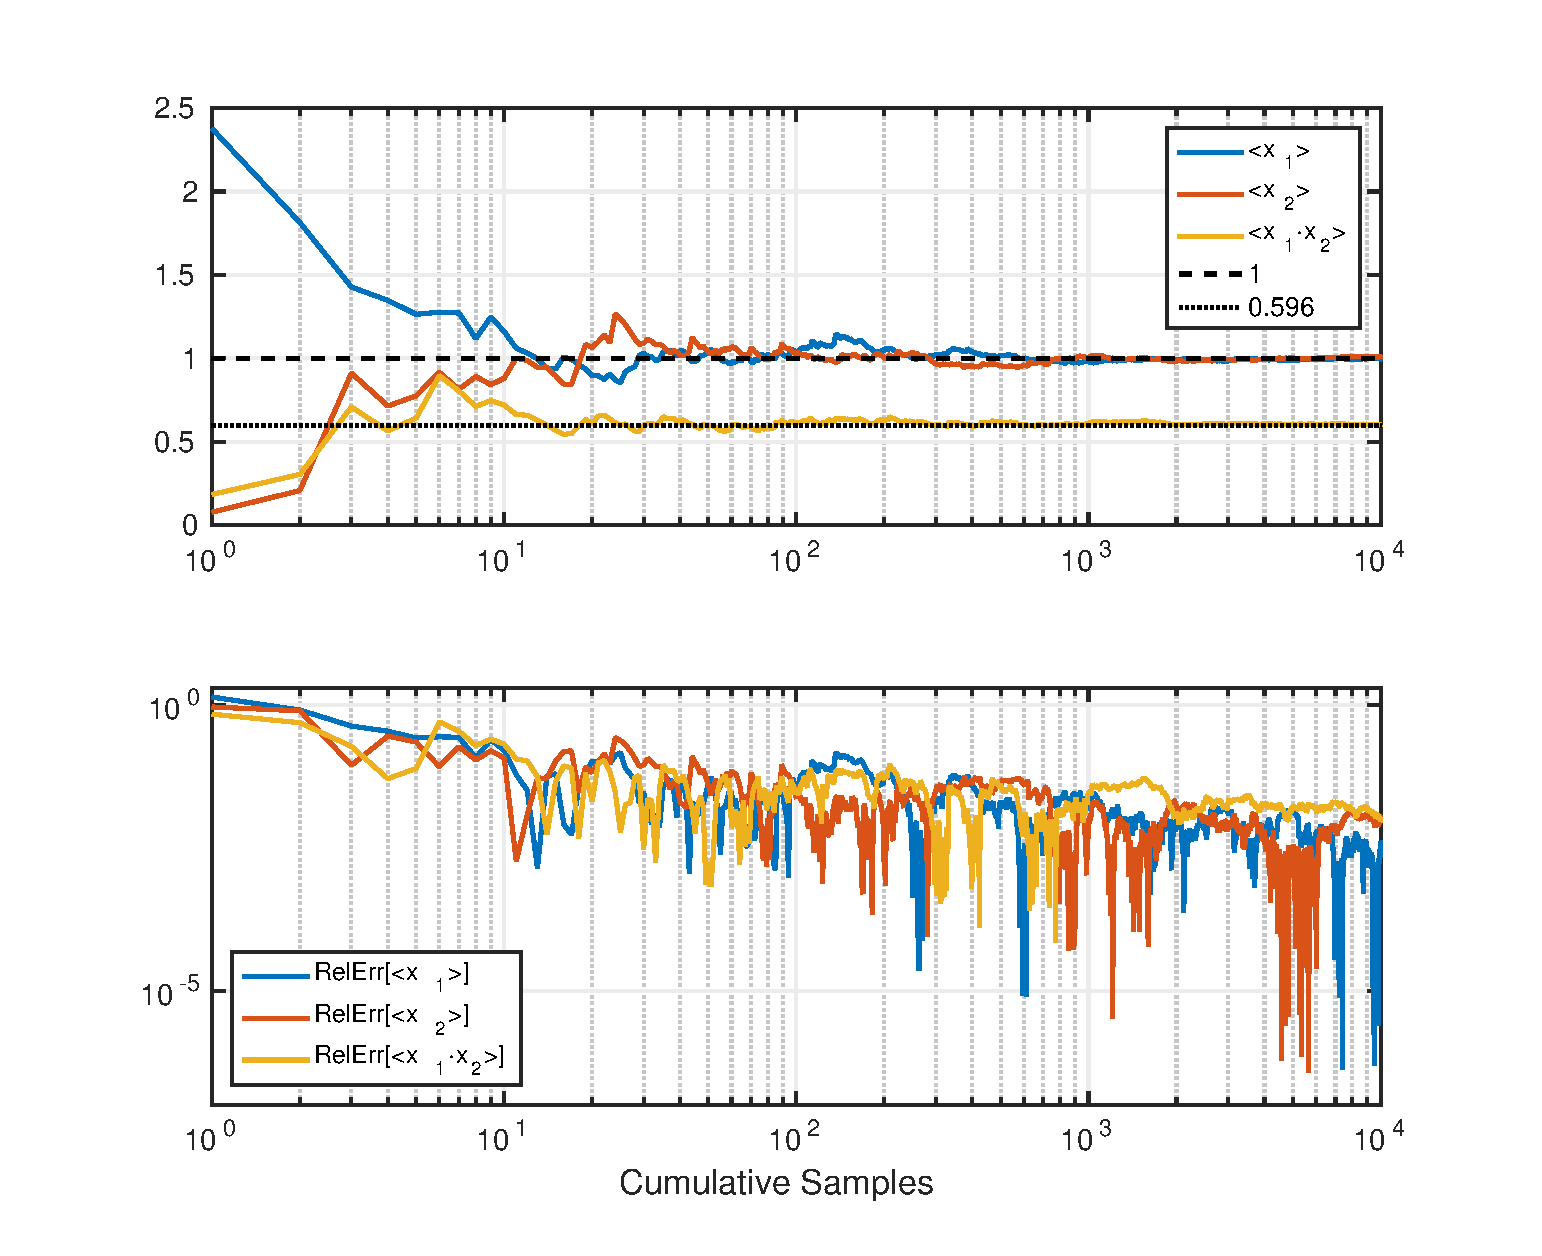
\includegraphics[width=\textwidth, trim={1in 0 1in 0}]{Prob1.eps}
\caption{Expectation values of various functions of $x_1$ and $x_2$, using the first $n$ cumulative samples. Analytical expectation values plotted to show convergence, as well as relative error.}
\label{fig:prob1}
\end{figure}

%%%%%%%%%%%%%%%%%%%%%%%%%%%%%%%%%%%%%%%%%%%%%%%%%
%%%%%%%%%%%%%%%%%%%%%%%%%%%%%%%%%%%%%%%%%%%%%%%%%
\section*{Problem 2} %%%%%%%%%%%%%%%%%%%%%%%%%%%%
%%%%%%%%%%%%%%%%%%%%%%%%%%%%%%%%%%%%%%%%%%%%%%%%%
%%%%%%%%%%%%%%%%%%%%%%%%%%%%%%%%%%%%%%%%%%%%%%%%%

This problem concerns a derivation from scratch of the Bayesian MAP estimate of a random variable $V$, assuming a Gaussian prior $V \sim N(V_0, \sigma_0^2)$. Further details are worked by hand on the attached sheets.

%%%%%%%%%%%%%%%%%%%%%%%%%%%%%%%%%%%%%%%%%%%%%%%%%
%%%%%%%%%%%%%%%%%%%%%%%%%%%%%%%%%%%%%%%%%%%%%%%%%
\section*{Problem 3} %%%%%%%%%%%%%%%%%%%%%%%%%%%%
%%%%%%%%%%%%%%%%%%%%%%%%%%%%%%%%%%%%%%%%%%%%%%%%%
%%%%%%%%%%%%%%%%%%%%%%%%%%%%%%%%%%%%%%%%%%%%%%%%%

Bloop!

%%
%% DOCUMENT END
%%
\end{document}
